% This is LLNCS.DEM the demonstration file of
% the LaTeX macro package from Springer-Verlag
% for Lecture Notes in Computer Science,
% version 2.4 for LaTeX2e as of 16. April 2010
%
\documentclass{llncs}
%
%\usepackage{makeidx}  % allows for indexgeneration
\usepackage{graphicx}
\graphicspath{ {./figures/} }
%
\begin{document}

\title{Automatic Estimation of the Optic Nerve Sheat Diameter from Ultrasound Images}
%
\titlerunning{Automatic Optic Nerve Sheat Diameter Estimation} % abbreviated title (for running head)
%                                     also used for the TOC unless
%                                     \toctitle is used
%
\author{
Samuel Gerber,
Maeliss Jallais,
Stephen Aylward
}

%
\authorrunning{S. Gerber, M. Jallais and S. Aylward} % abbreviated author list (for running head)
%
%%%% list of authors for the TOC (use if author list has to be modified)
%\tocauthor{}
%
\institute{Kitware Inc, Carrboro NC 27510, USA,\\
\email{samuel.gerber@kitware.com}
}

\maketitle              % typeset the title of the contribution

\begin{abstract}
\end{abstract}
%
\section{Introduction}
Portable ultrasound technology is well suited for the development of automated
diagnostics systems that enable emergency responders to quickly assess the
severity of a patient's injuries at accidents. Such light-weight portable
automated systems can be employed in remote environments in which expert medical
imaging personnel and advanced imaging equipment are not readily available.
 
This paper considers the application of a point-of-care, computer-assisted
ultrasound system for in-field traumatic brain injury (TBI) assessment via the
detection of increased intracranial pressure. Delayed treatment of increased
intracranial pressure can cause temporary or permanent brain damage or even
long-term coma and death. For example, it has been shown that acute subdural
hematomas in severe TBI patients cause significant increase in intracranial
pressure, are associated with 90\,\% mortality if detected and treated more than
4 hours after injury, and yet are associated with only 30\,\% mortality if
detected and treated earlier~\cite{Se1981}.

In a clinical setting, a non-invase appraoch to measure intracranial pressure is
by ocular ultrasound. From the ocular ultrasound image the physicians manually
measures the diameter of optic nerve sheath at a location 3\,mm behind the retina.
Acquiring such images and making these measurements is challenging and time
consuming task. We porpose to automate the process of measuring the diameter of
the optic nerve sheath and integrate within a portable ultrasound system to
automatically report elevated intracranial pressure without the need of manually
measuring the optic nerve sheath diameter. The ultimate goal is a system that is
easy to use and does not require expert personnel or specific trainng to
diagnose TBI.    

\section{Related Work}


\section{Algorithm}
We propose a two step approach to automate the measurement of the optic nevre
sheath diameter. At a high level, the algorithm proceeds by locating the orb of
the eye through registration of an ellipse with the largest dark circle in the
image data. From the ellipse an approximate location of the optic nerve is
constructed and used to fit two bars to the walls of the optic nerve. This
high-level description leaves out several intermediate steps such as those
involving image smoothing, morphological operations, and distance transforms,
that are required to achieve good registration results. Figure~\ref{fig:fitted}
shows result of the fitting procedure and illustrates that the proposed
algorirthm is applicabale to a wide variety of images with differing quality.
\begin{figure}
\centering
\begin{tabular}{ccc}
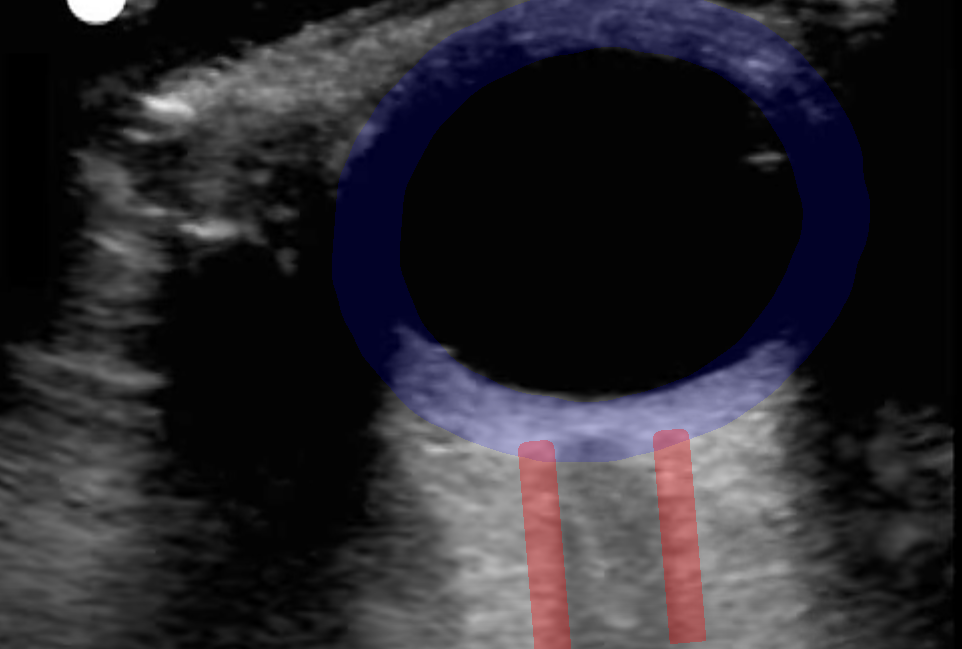
\includegraphics[height=1.5in]{003-overlay.png} &
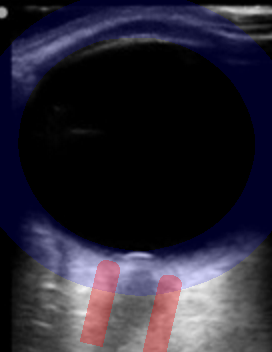
\includegraphics[height=1.5in]{009-overlay.png} &
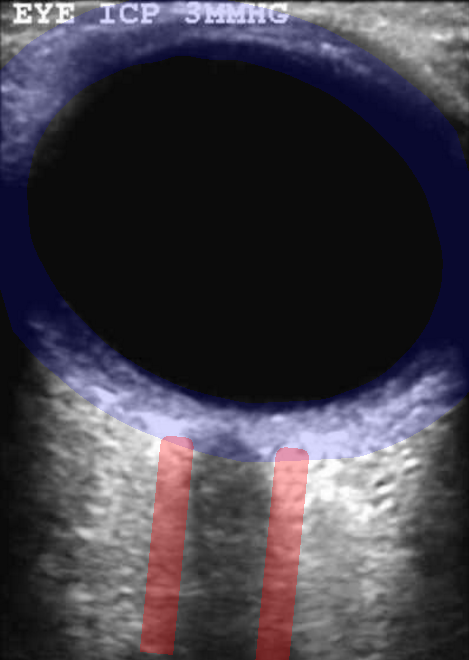
\includegraphics[height=1.5in]{023-overlay.png} 
\end{tabular}
\caption{
\label{fig:fitted}
Result of the proposed algorithm on three occular ultrasound images. The
overlays illustrate the registration results of the algorithm. The blue ellipse
delineates the location of they eye orb and the red bars are the result of
fitting the boundray of the accoustic shadow induced by the optic neve sheath.
}
\end{figure}

\subsection{Algorithm Details}
Here we briefly describe the individual image processing steps to achieve an
algorithm that performs a large variety of images from different types of probes
and differcens between subjects.

The first part of the algorithm is locating and estimating the size of the eye
and involves the following steps:
\begin{enumerate}
\item Estimate initial eye center and size
  \begin{enumerate}
  \item Gaussian smoothing
  \item Binary Thresholding
  \item Morphological closing
  \item Distance transform. 
  \item The maximum distance and its location of the distance transfrom provide inital radius
        and inital center of the eye orb. 
  \end{enumerate}
\item Refine intial estimates
  \begin{enumerate}
  \item Distance transform over vertical image strip of width 20 pixels
        around the intial eye center location estimate provides an intial
        minor ellipse radius.
  \item Distance transform over horizontal image strip of width 20 pixels 
        around the intial eye center location estimate provides an inital major
        ellipse radius.
  \end{enumerate}
\item Gaussian smoothing, threshold and rescale
\item Create an binary ellipse annulus with the intial estimates of the minor and
      minor axis of width $0.2$ times the major axis with center located at the
      intial eye location estimate.
\item Register ocular ultrasound (moving image) to ellipse image (fixed image)
      under an affine transform with a masked mean squaered error metric. The
      mask is an ellipse that encomposses the ellipse annulus on the fixed
      image. The affine transfrom is centered on the ellipse center.
\item Refine eye center and major and minor estimates applying the transform to
      the minor and major axiis vectors and the center point.
\end{enumerate}
\begin{figure}
\centering
\begin{tabular}{ccccc}
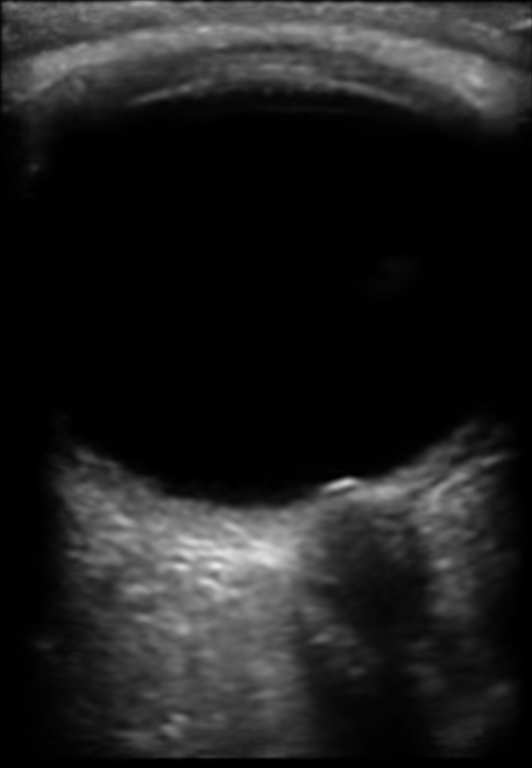
\includegraphics[height=1.32in]{019.png} &

\includegraphics[height=1.32in]{019-eye-smooth.png} &

\includegraphics[height=1.32in]{019-eye-distance.png} &         

\includegraphics[height=1.32in]{019-eye-moving.png} &
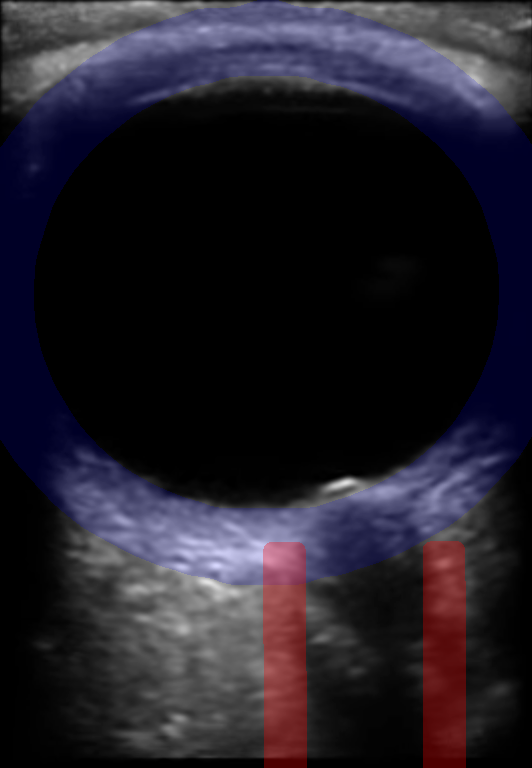
\includegraphics[height=1.32in]{019-overlay.png}\\
(a) & (b) & (c) & (d) & (e)
\end{tabular}
\caption{
\label{fig:algorithm-eye}
Intermediate steps to locate the ye orb.
}
\end{figure}

The location of they orb provides an approximate region for locating the
accoustic shadow of the optic nerve for the second part, estimating the width of
teh accoustic shadow of the optic nerve sheath, of the algorithm. Estimating the
width of the accoustic shadow involves the following steps:
\begin{enumerate}
\item Extract optic nerve region below the eye using the eye location and size estimates
\item Preprocess ( Gaussian smoothing, Rescale individual rows )
\item Compute initial center and width estimates
  \begin{enumerate}
  \item Binary threshold, Morphological opening, Add vertical border and small horizontal border, Distance transform
  \end{enumerate}
\item Scale rows on each side of the optic nerve center independently
\item Refine initial center and width estimates
  \begin{enumerate}
  \item Binary threshold, Morphological opening, Add vertical border and small horizontal border, Distance transform
  \end{enumerate}
\item Register U-profile image to processed image with a similarity transform
  \begin{enumerate}
  \item Use initial center and width to create U-profile image
  \item Mask cost function
  \end{enumerate}
\item Refine width estimates through the affine transform
\end{enumerate}
\begin{figure}
\centering
\begin{tabular}{cccccc}
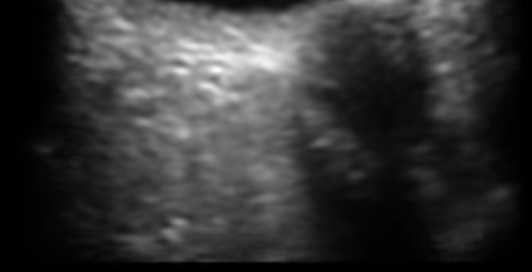
\includegraphics[height=0.36in]{019-nerve.png} &
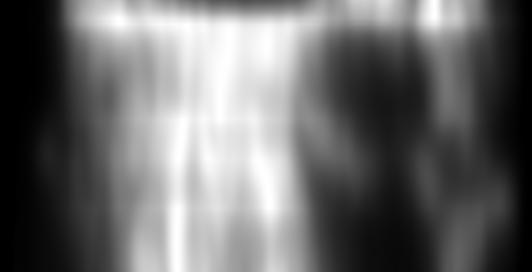
\includegraphics[height=0.37in]{019-nerve-smooth.png} &

\includegraphics[height=0.36in]{019-nerve-distance.png} &
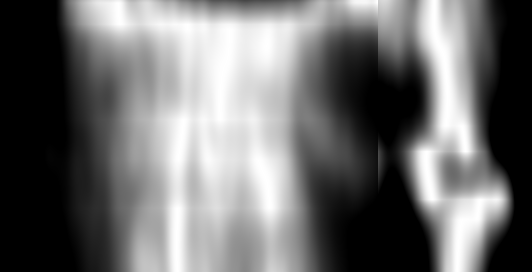
\includegraphics[height=0.36in]{019-nerve-scaled.png} &

\includegraphics[height=0.36in]{019-nerve-thres.png} &         

\includegraphics[height=0.36in]{019-nerve-moving.png} \\         
(a) & (b) & (c) & (d) & (e) & (f)
\end{tabular}
\caption{
\label{fig:algorithm-nerve}
Intermediate steps to fit the accoustic shadow of the optic nerve sheath.
}
\end{figure}

\subsection{Interactive Graphical User Interface}
Our algorithm reports estimates of the optic nerve sheath diameter in near real
time as an ultrasound probe is swept across the closed eye of a patient. 
This algorithm is now integrated into a user-friendly interface and performs
estimates at 4 frames per second. Depending on the ultrasound probe, the
algorithm can be simplified by skipping the eye estimation step to run at
around 20 frames per second.
\begin{figure}
\centering
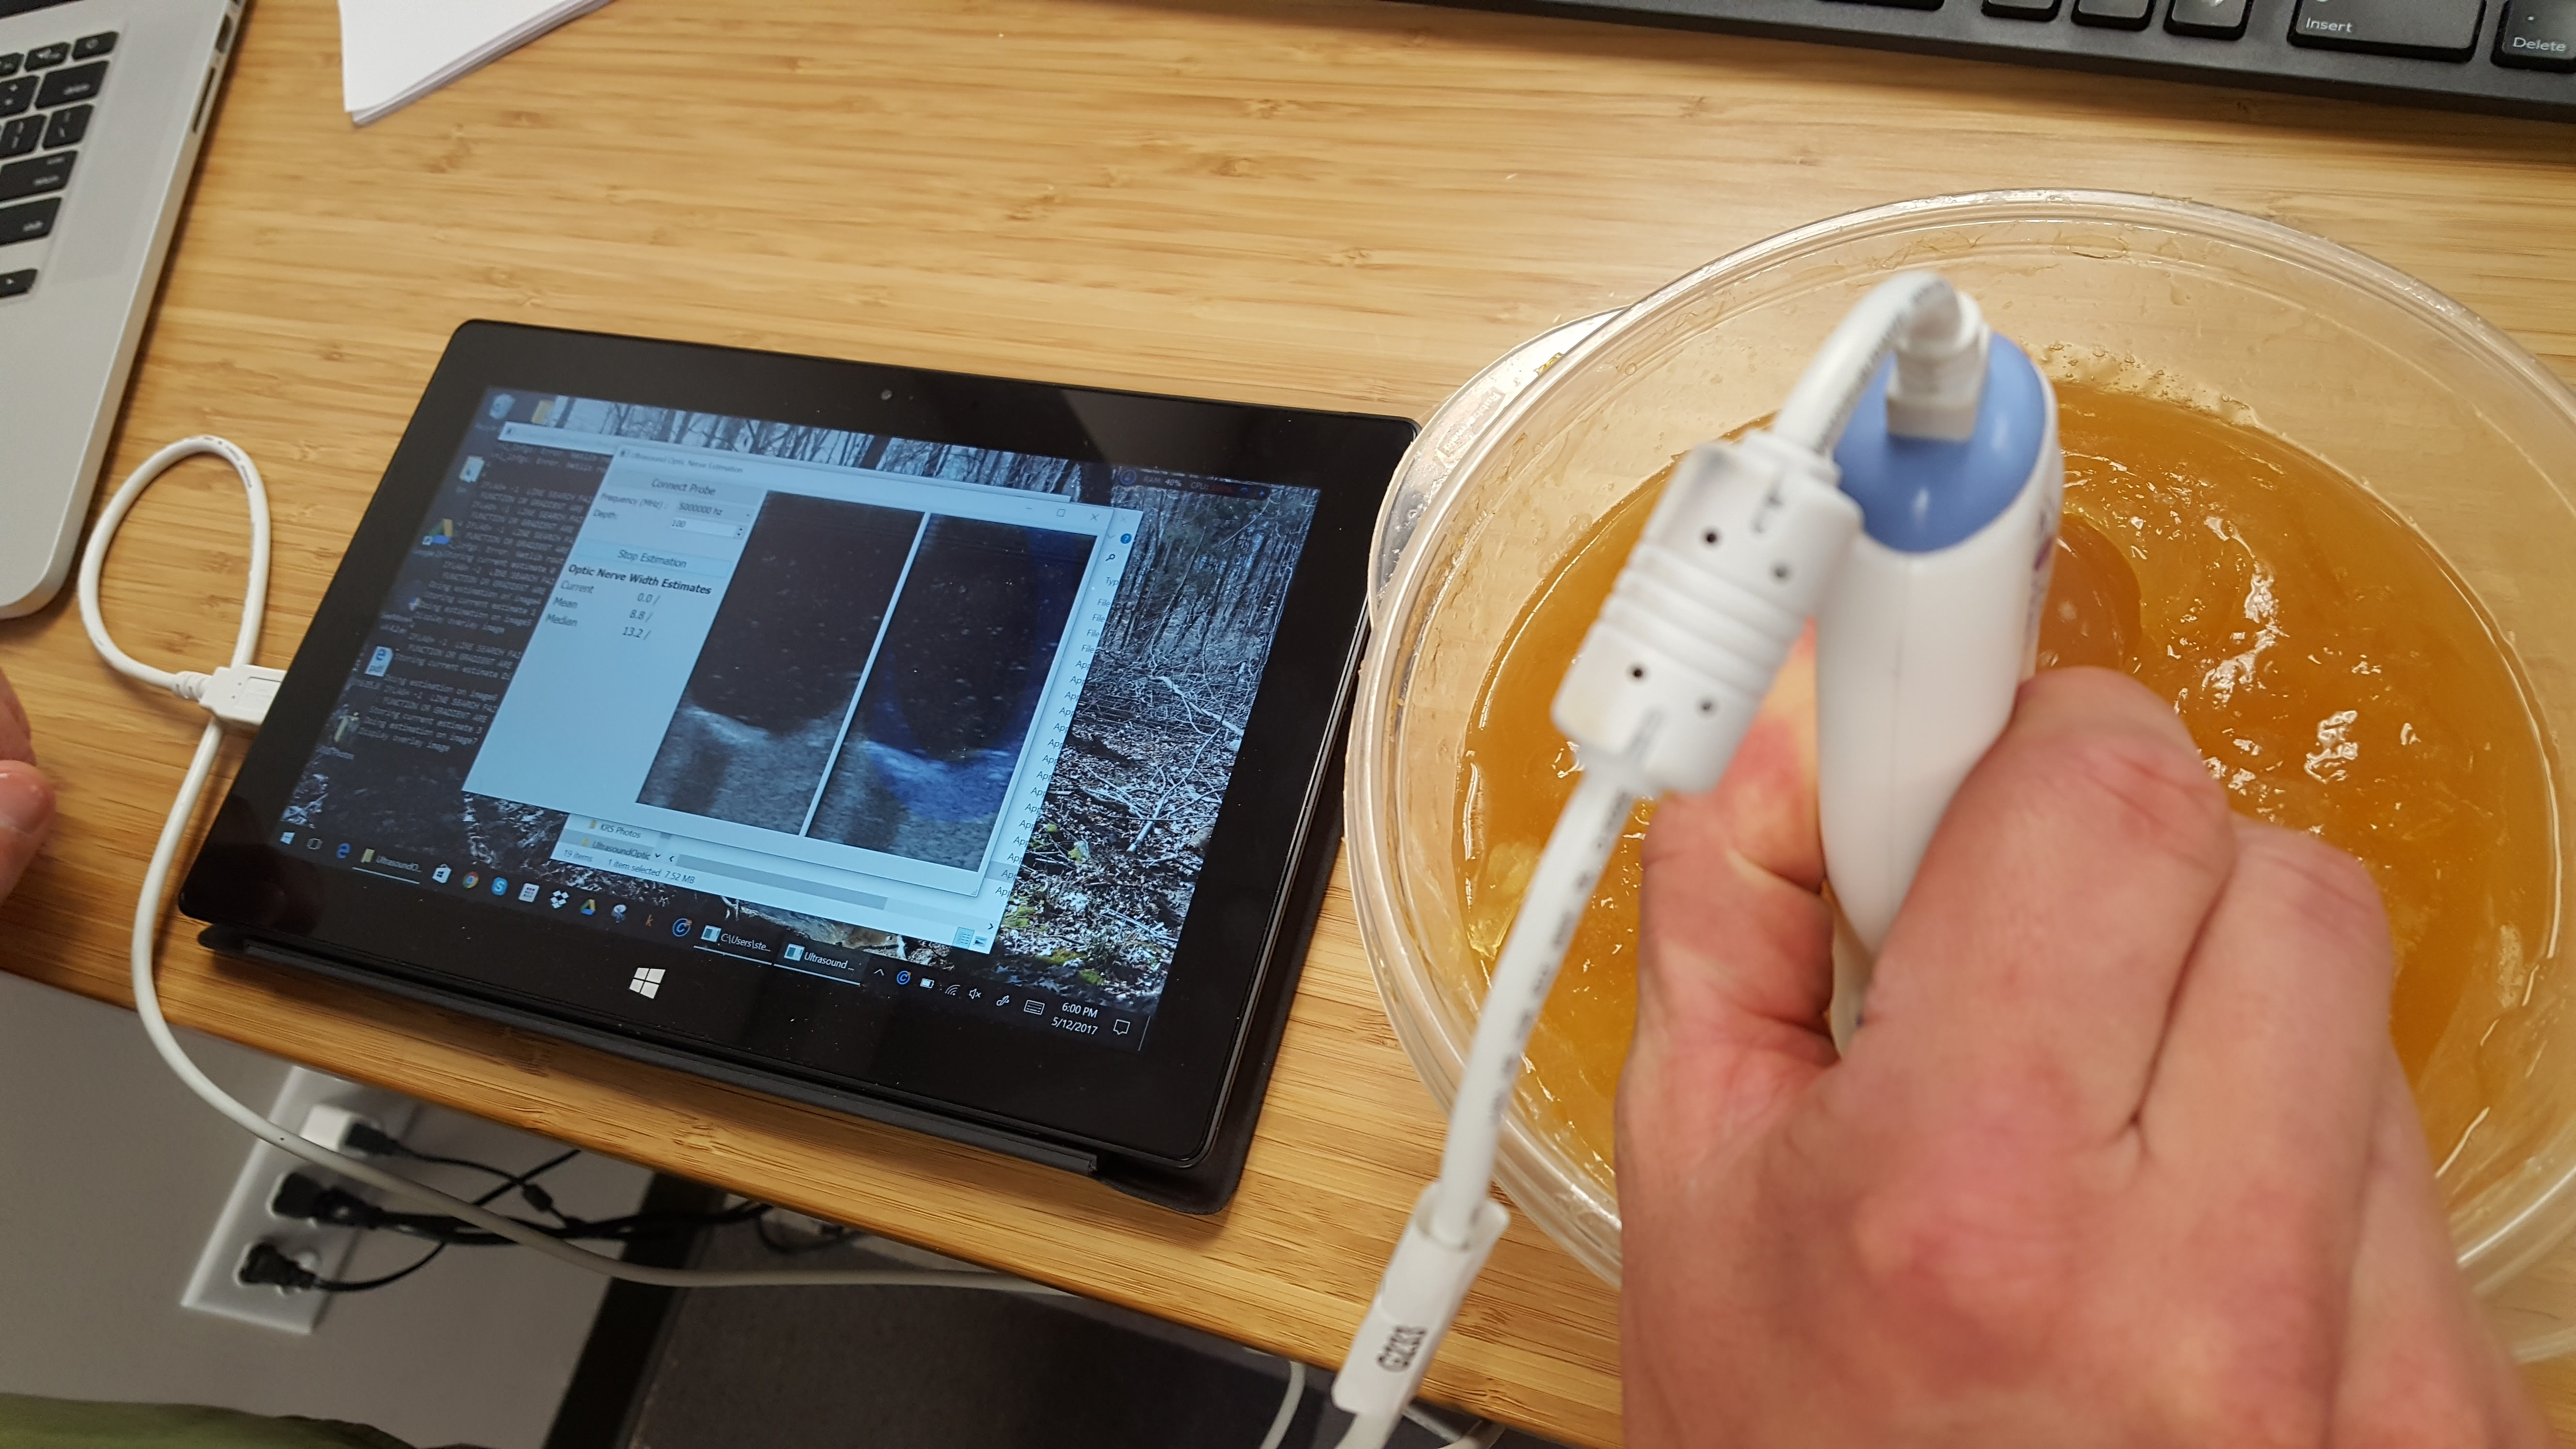
\includegraphics[width=0.85\linewidth]{gui.jpg} 
\caption{
\label{fig:gui}
Graphical user interface to image an eye phantom on a windows table connected to
a USB ultrasound probe from Interson at interactive framerates. 
}
\end{figure}

\section{Evaluation}

\subsection{Comparison to Manual Estimation}
To evaluate the quality of the estimates we had 13 volunteers ranging from
Kitware engineers to medical professionals annotate 23 ultrasound images.  The
image below shows a linear fit of the automatic estimated diameter from two
different parameter settings of the algorithm as compared to a medical
professional. The automatic estimates had an R2 of around 0.9 and 0.8,
respectively. The mean intra correlations among medical professionals was 0.84.
Thus, on this small sample size the automatic estimates perform on par with
medical experts. The correlation among experts matches results of previous
studies.

\subsection{Gel Phantom Study}
For additional evaluation of the performance of the algorithm we built a
phantom from gelatine in which 3D-printed “optic nerves” (plastic discs) of
known diameter can be embedded under gelatine orbs and imaged, producing
ultrasound images that look closely resemble clinical ocular ultrasound images.
The deatils for construction of the phantom are describd in~\cite{Ze2014}.
\begin{figure}
\centering
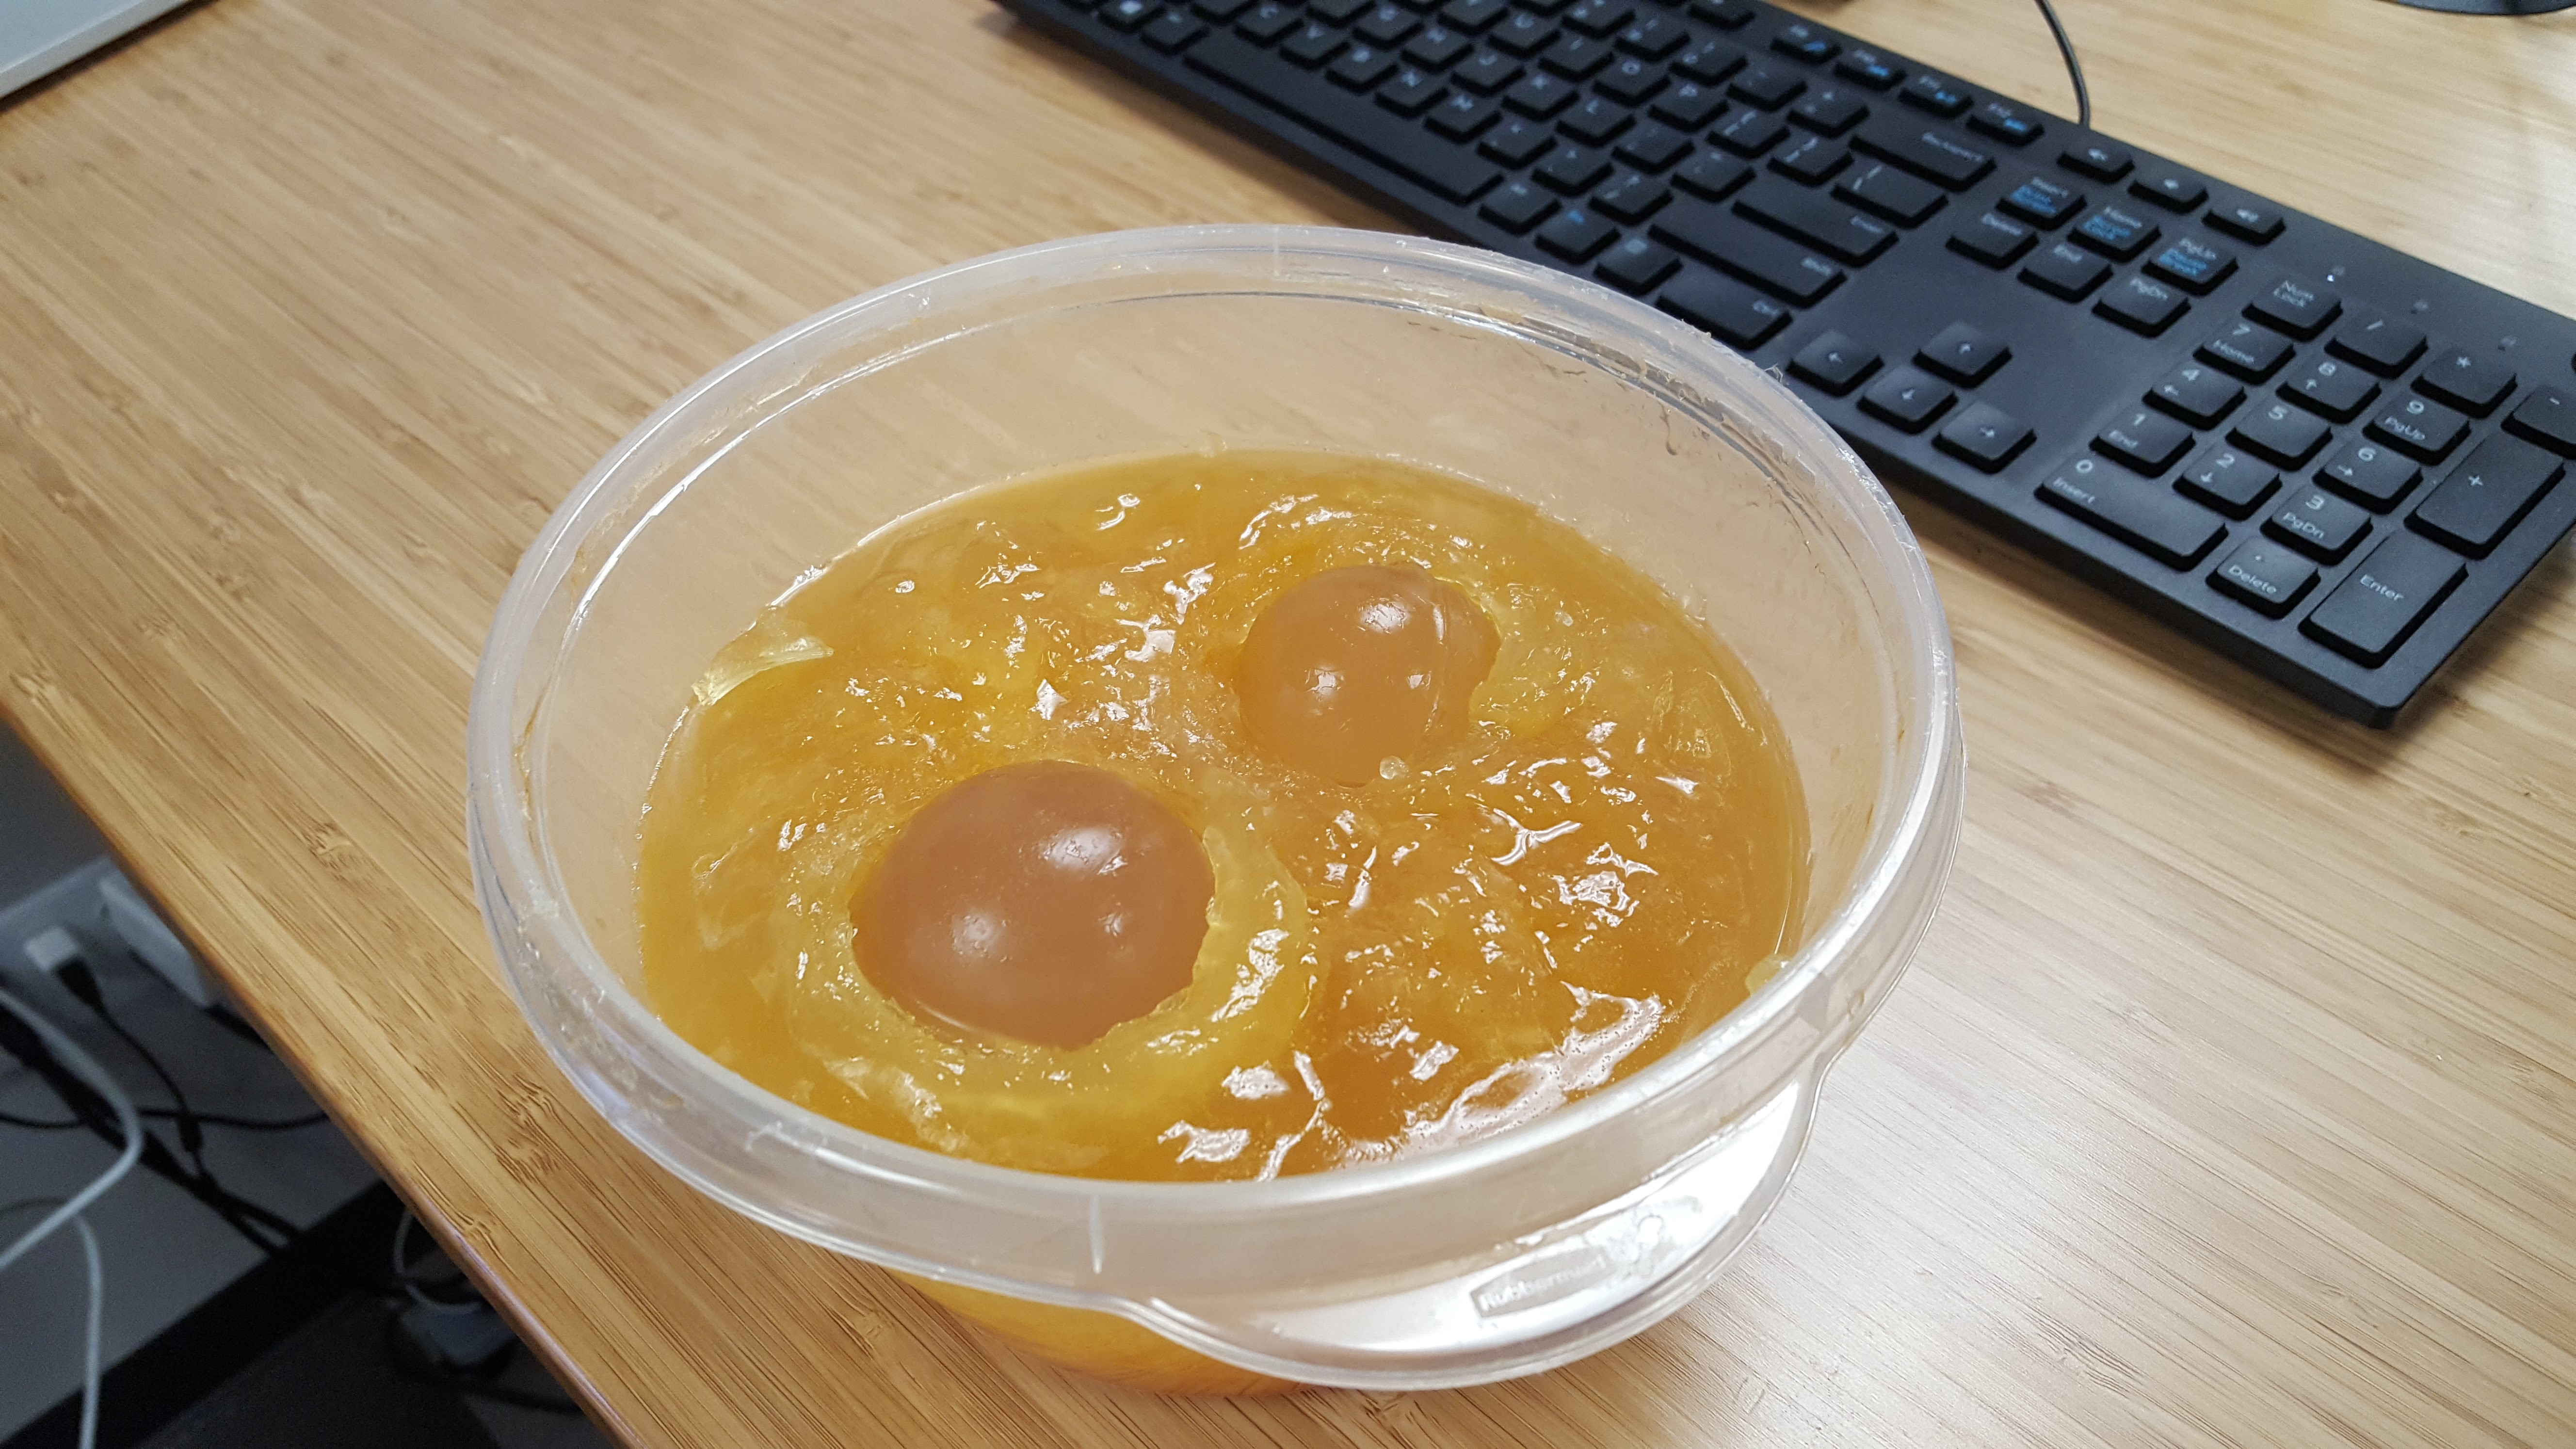
\includegraphics[width=0.85\linewidth]{phantom.jpg} 
\caption{
\label{fig:phantom}
Gelatine phantom for aquiring ultrasound images with know ground truth optic
nerev sheath diameters. The images from the phantom are very realistic
approximation to images aquired through occular ultrasound. 
}
\end{figure}

The goal of this evaluation is to check if an accurate estimate of the optic
nerve is possible with the proposed algorithm. In this controlled setting we
first located the optic nerve using the ultrasound. Once a good image of the
optic nerve was achieved the automatic estimation process was started and run
interactively for about 10 seconds which resulted in approximately 40 to 50
optic nerve sheath diameter estimates. The table below shows that the means of
the automatic estimates are within less than +/- 0.5mm  with a relatively tight
distribution of estimates around the ground truth diameter. A study on
intra-operator variations on the same type of phantom, reports standard
deviations of the measurements ranging from 0.25 to 0.6 mm depending on
diameter size.  

\section{Conclusion}
The results presented indicate that the algorithm performs well in a controlled
setting.  A retrospective analysis of clinical images indicate that our system
performs similar to an expert, and a phantom study using 3D printed optic
nerves of known diameter suggests that our system is accurate.

The next step is to integrate an image quality estimation algorithm, so that
high quality images of the optic nerve can be automatically identified as a
probe is swept over the eye. This will eliminate the need for the operator to
view, interpret, or make measurements on an ultrasound image when using it to
assess a dilated optic nerve sheath, as indicative of increased intracranial
pressure. Ultimately, we aim for a system that can be used by novice operators
with minimal ultrasound experience. The system will report when a sufficient
image has been acquired, and it will automatically determine if the diameter of
the optic nerve is greater than 5mm, thereby indicating increased intracranial
pressure associated with mild or more severe TBI [4].

The long term goal of Kitware is to develop a lightweight portable ultrasound
system that, in addition to automated diagnosis of TBI, includes automatic
diagnosis tools for pneumothorax (detached lung) and internal bleeding.

%
% ---- Bibliography ----
%
\begin{thebibliography}{}
%
\bibitem[Du2012]{Du2012}
Dubost, Clément, et al. 
Optic Nerve Sheath Diameter Used as Ultrasonographic Assessment of the Incidence
of Raised Intracranial Pressure in PreeclampsiaA Pilot Study.  
The Journal of the American Society of Anesthesiologists 116.5 (2012): 1066-1071.

\bibitem[Jo2016]{Jo2016}
Johnson, Garrett GRJ, et al. 
Estimating the accuracy of optic nerve sheath diameter measurement using a
pocket-sized, handheld ultrasound on a simulation model.  Critical Ultrasound
Journal 8.1 (2016): 18.

\bibitem[Ma2015]{Ma2015}
Maissan IM , Dirven PJ , Haitsma IK , Hoeks SE , Gommers D , Stolker RJ 
Ultrasonographic measured optic nerve sheath diameter as an accurate and quick
monitor for changes in intracranial pressure. 
J Neurosurg. 2015 Sep;123(3):7437

\bibitem[Se1981]{Se1981}
Seelig, John M., et al. 
Traumatic acute subdural hematoma: major mortality reduction in comatose
patients treated within four hours.
New England Journal of Medicine 304.25 (1981): 1511-1518.

\bibitem[Ze2014]{Ze2014}
Zeiler, F. A., et al. 
A unique model for ONSD Part II: inter/intra-operator variability. 
Can J Neurol Sci 41 (2014): 430-435.


\end{thebibliography}

\end{document}
